\documentclass[article]{llncs}

\setcounter{tocdepth}{2}
\setcounter{secnumdepth}{2}
\usepackage[a4paper,left=3cm,right=3cm,top=2.5cm,bottom=2.5cm]{geometry}
\usepackage{float}
\usepackage{amsmath,amssymb}
\usepackage{colortbl}
\usepackage{flafter} 
\usepackage{minted}
\usepackage{graphicx}


\begin{document}
%
\graphicspath{ {./images/} }
\title{Advanced Machine Learning, Deep Learning, NLP \& Graphical Models}
%
%
\author{Ryan Vaz}
\institute{Hunter College}
%
%
\maketitle 
%
\begin{abstract}
This PDF is a collection of lecture notes from the Statistics 72556 class at Hunter College with some brief simplifications and details regarding how to approach Machine Learning from a Statistical POV. A firm grasp of Python Programming, Statistics, and Matrix/Linear Algebra is assumed. I'll try to minimize the usage of Calculus however some understanding will help certain topics.
\end{abstract}
%
\begingroup
\let\clearpage\relax
\tableofcontents*
\endgroup
%
\section{Lecture 1 - ANN}
\subsection{Machine Learning Problems}

\subsubsection{Unsupervised Learning} A problem where only the features are observed.

\subsubsection{Supervised Learning} A problem in which both the features and the target are observed. We can further classify supervised learning into two categories...

\subsubsection{Regression} A case of supervised learning where the variable we are studying is continuous/numerical

\subsubsection{Classification} A case of supervised learning where the variable we are studying is categorical

\begin{table}
\caption{Examples of different machine learning problems and classifications}\label{tab1}
\begin{tabular}{|l|l|}
\hline
Problem Type &  Example \\
\hline
Unsupervised &  {Market segmentation where we divide customers into groups based on their characteristics}\\
\hline
Regression &  {Predicting the value of the DOW in 6 months} \\
           & {Predicting the value of a given house based on various inputs}\\
\hline
Classification & {Will the DOW be up (T) or down (F) in 6 months?}\\
               & {Is this email a spam(T) or not(F)?} \\
\hline
\end{tabular}
\end{table}

\subsection{Basic Neural Networks}

\subsubsection{Artificial Neural Networks(ANNs)} A neural network is a computing system that is inspired by biological neural networks that make up the brain. They consist of multiple connected units called artificial neurons or linear threshold units.

\subsubsection{Linear Threshold Unit(LTU)} A single artificial neuron that calculates the net output from a series of inputs\\ It uses inputs(x) and weights(w) to calculate a weighted sum \\ That value is then applied to a binary step function which turns the result into a Boolean value.
\begin{theorem}[Weighted Sum]\\
    $z = w_1x_1+w_2x_2+...+w_kx_k = $ \textbf{x}$^T$\textbf{w}
\end{theorem}
\begin{theorem}[Step Function]\\
    \text{step(z)=}
    $\begin{cases}
        0 & \text{if } z < 0\\
        1 & \text{if } z \geq 0
    \end{cases}$
\end{theorem}
\begin{figure}[H]
\centering
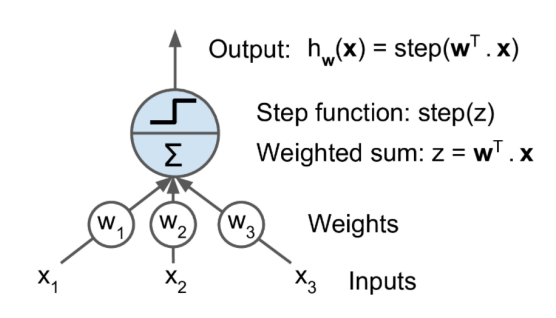
\includegraphics[scale=0.5]{fig1.PNG}
\caption{Example of a LTU.} \label{fig1}
\end{figure}
To summarize a single LTU: It takes in data from input layer and calculates output by multiplying it with the corresponding weight then summing it together and sending it through a step function(Binary Step Function in this case).

\subsubsection{Perceptron} A neural network formed from a single layer of LTUs\\
Each LTU is connected to all the input neurons along with an extra input neuron that is always 1(bias neuron). This bonds the Input Layer to the Output Layer.\\These Perceptrons can output several values(Multioutput Classifier).
\begin{figure}[H]
\centering
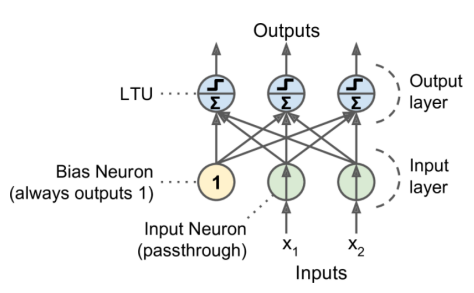
\includegraphics[scale=0.55]{fig2.PNG}
\caption{Example of a Dense Perceptron.} \label{fig2}
\end{figure}
\noindent If all the neurons in a layer are connected to every neuron in the previous layer, its a
dense layer
 \begin{theorem}[Output of a Dense Layer]\\
    $h_{W,b}(X) = \phi(XW + b)$
\end{theorem}
$\phi$ - activation function\\
X - inputs, W - weights, b - bias vector
\subsection{Deep Neural Networks}
\subsubsection{Perceptron Training} It's commonly believed that when biological neurons trigger others, it reinforces the connection between these two, the same logic is what's used for perceptrons.\\ To train perceptrons, they're given a training instance and it makes a prediction.\\ When it makes a WRONG prediction, this reinforces the connection between the inputs that would have contributed to a correct prediction.\\ This can be expressed mathematically as follows:
\begin{theorem}[Weights Update]\\
    $w_{i,j}^{\text{next step}} = w_{i,j} + \eta(y_j - \hat{y}_j)x_i $
\end{theorem}
$w_{i,j}$ is the connection weight between the i-th input neuron and the j-th output neuron\\
$x_i$ is the i-th input value of the current training instance\\
$\hat{y}_j$ is the output of the j-th output neuron for the current training instance\\
$y_j$ is the target output of the j-th output neuron for the current training instance\\
$\eta$ is the learning rate

\subsubsection{Deep Neural Networks(DNNs)} When a perceptron has multiple layers of LTUs(or hidden layers) that are fully connected to the next layer with a bias on each level, we call that a Multilayer Perceptron(MLP) or Deep Neural Network(DNN).
\begin{figure}[H]
\centering
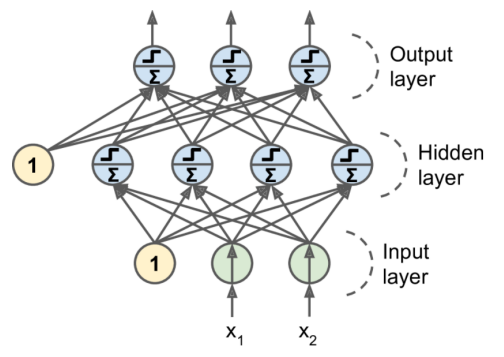
\includegraphics[scale=0.55]{fig3.PNG}
\caption{Example of a DNN.} \label{fig3}
\end{figure}
\subsection{Error Backpropagation Learning Algorithm}
\noindent The next set of topics is going to be significantly harder, so if you want to get the spark notes and skip to the coding section, they go as follows: in order to train DNN's a backpropagation training algorithm is used, which is basically gradient descent using reverse-mode autodifferentiation.\\ \\
Note: This section is going to be different in that we will simulate each step of the algorithm

\subsubsection{Initialization} The weights of the input layer are initialized with random small values.
\subsubsection{Forward pass} The input layer is provided and the neural network begins processing the data. The difference between expected and actual value is provided directly to the backwards pass step.
\subsubsection{Reverse Pass} This step computes how much each neuron in the last hidden layer contributed to each output neuron’s error and it tweaks the weights according to a gradient descent(coming soon!). \\

\noindent It then repeats the initialization, forward pass and backwards pass which is why this whole process is called backpropagation, or backprop for short as it propagates the error back to the weights of the neurons that contributed to the error. \\

Now the question remains, how do we minimize this error function?
\subsection{Gradient Descent(GD)}
Yes, Gradient Descent gets it's whole own section, mad? Stay mad.
\subsubsection{Definition}
GD is a optimization algorithm that starts with a random value on a graph and will try tweaking the parameters in order to minimize a cost/error function\\
By using GD, we can find the minimum amount of error to best use with our DNN.\\
\begin{figure}[H]
\centering
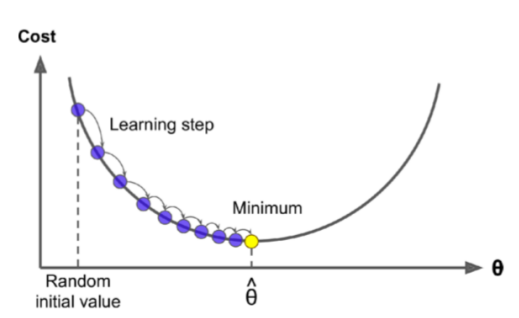
\includegraphics[scale=0.60]{fig4.PNG}
\caption{Example of Gradient Descent.} \label{fig4}
\end{figure}
\subsubsection{Learning Rate($\eta$)}
Learning rate will determine the size of the steps. If it's too small, it won't be able to get a solution in a reasonable amount of iterations. If it's too big, it may skip the final result entirely and diverge!\\
Learning rate is so important can make or break our code, thus it is a hyper-parameter. Our code has other hyper-parameters that we will address later on.
\begin{figure}[H]
\centering
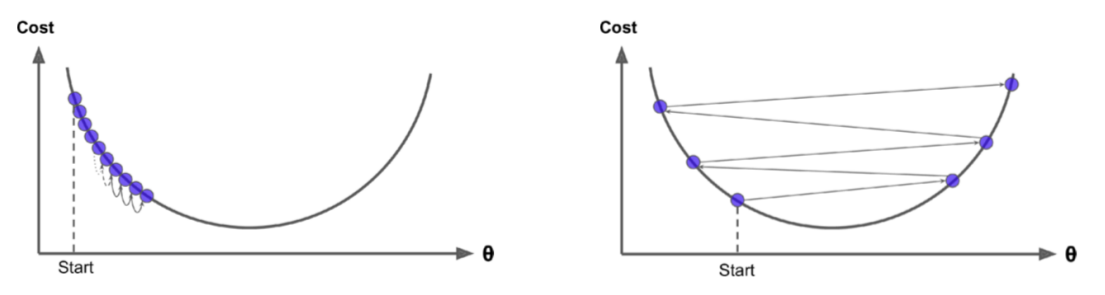
\includegraphics[scale=0.50]{fig5.PNG}
\caption{Example of bad learning rates.} \label{fig5}
\end{figure}
\subsubsection{Math}
Problem: Minimize f(w) - weight/error function\\
iterative solution: $w_{k+1} = w_k - \gamma_k \nabla f(w_k)$\\
$w_{k+1}$ = next iteration \\
$w_{k}$ = current iteration \\
$\gamma_k$ = step size \\
$\nabla f(w_k)$ = gradient of f\\
One such example is our linear regression problem, let's switch w with $\theta$\\
$\hat{y} = \theta_0 + \theta_1x_1+\theta_2x_2+...+\theta_nx_k = h_\theta(x) = $ \textbf{$\theta$}$^T$\textbf{w}\\
We need to find $\hat{\theta}$ which is the minimizes the criterion(loss)\\
$f(\lambda_k) = MSE(X, h_\theta) = \frac{1}{m}\sum^m_{i=1}(\theta^Tx^{i}-y^i)^2, \nabla f = \frac{2}{m}X^T(X\theta-y)$\\
Gradient Descent Step Equation\\
$\theta^{nextstep} = \theta - \eta\nabla_\theta MSE(\theta)$\\
where\\
$\nabla_\theta MSE(\theta) = \begin{pmatrix}
\frac{\partial}{\partial \theta_0} MSE(\theta)\\
\frac{\partial}{\partial \theta_1} MSE(\theta)\\
: \\
\frac{\partial}{\partial \theta_n} MSE(\theta)
\end{pmatrix} = \frac{2}{m} X^T(X\theta-y)$\\
Implementation in code:\\
\begin{minted}{python}
eta = 0.1 #learning rate
n_iterations = 1000
m = 100

theta = np.random.randn(2,1)

for iter in range(n_iterations):
    gradients = 2/m * X_b.T.dot(X_b.dot(theta) - y)
    theta -= (eta * gradients)
\end{minted}

\section{Lecture 2 - MLP Architecture}
\subsection{Math}
\subsubsection{MLP as a Composite Function}
Imagine each layer of the Neural Network is a function, then we can say that function n maps to function k with the invertable linear map $f: R^n \xrightarrow{} R^k$ where f is expressed as the following
\begin{theorem}
    $f(x) = g \circ f_N \circ f_{N-1} ... \circ f_2 \circ f_1(x), \-\ \-\ \-\ \-\  f_i : R^{i-1} \xrightarrow{} R^i \\ $ \text{where} $ f_i(x) = \sigma (w_ix+b_i), i = 1,2,...N \\ \implies f(x) = g(\sigma(...(\sigma(w_2\sigma(w_1x+b_1)+b_2)+...+b_N)$
\end{theorem}
Where $\sigma$ is a non-linear activation function and g(x) is the linear decision function.
\subsubsection{Autodiff}
s.p.z. we have a function that maps n dimensional values to a scalar output, and we have $x_1, x_2, ... , x_n$ as inputs, and $x_{n+1}, ... , x_{N-1}$ as intermediate values, and $x_N$ to be the final value.  \\
Example problem: Compute $f(x), L(f(x),y),$ and $dL/dw_i$
\begin{enumerate}
    \item Input \textbf{x}
    \item Set $v_{1,..n} \xleftarrow{} x$
    \item For i = n+1, n+1, ..., N:
    \item[] \centering $v_i \xleftarrow{} \sigma_i(w_i \cdot v_{Pa(i)})$
    \item[] \centering $v'_i \xleftarrow{} \sigma'_i(w_i \cdot v_{Pa(i)})$
    \item \raggedright Set $L \xleftarrow{} L(f,y)$
    \item Compute $\frac{dL}{df}$
    \item Initialize $\frac{dL}{dv_i} \xleftarrow{} 0$
    \item For m = 1, 2, ..., M:
    \item[] \centering $\frac{dL}{dv_{N-M+m}} \xleftarrow[]{} \frac{dL}{df_m}$
    \item \raggedright For i = N, N-1, ..., n+1:
    \item[] \centering $\frac{dL}{dw_i} \xleftarrow{} \frac{dL}{dv_i} v' v_{Pa(i)}$
    \item[] \centering $\frac{dL}{dv_{Pa(i)}} \xleftarrow{} \frac{dL}{dv_{Pa(i)}} + \frac{dL}{dv_i} v' w_{i} $
\end{enumerate}

\subsection{Hyperparameters}
\subsubsection{Hyperparameter Examples}
\begin{enumerate}
    \item $\#$ of hidden layers
    \item $\#$ of neurons per hidden layer
    \item Learning rate($\eta$)
    \item Optimizer
    \item Batch size
    \item Activation functions
\end{enumerate}

\subsubsection{Activation Functions}
\begin{enumerate}
    \item ReLU (most used)
    \item Hyperbolic tangent function (tanh)
    \item Logit function
    \item Sigmoid (not as good as ReLU, but biologically more accurate)
\end{enumerate}

\begin{figure}[H]
\centering
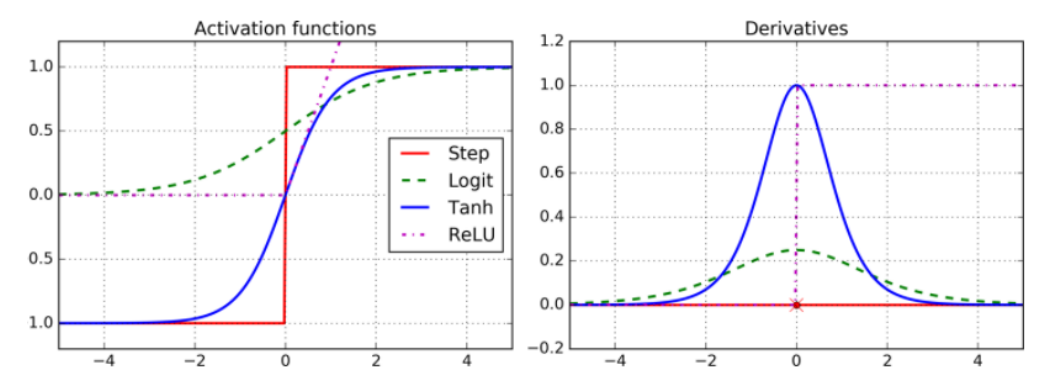
\includegraphics[scale=0.5]{fig6.PNG}
\caption{Comparison of activation functions.} \label{fig6}
\end{figure}

\subsubsection{Regression MLP Architecture}
When Using Regression, we do not need an activation function, and furthermore the loss function is normally Mean Square Error(MSE). Due to no activation function, it's easy to think of Regression MLP's as a MLP with the identity activation function.

\begin{table}[!htbp]
\caption{Examples of standard values for Hyperparameters}\label{tab1}
\begin{tabular}{|l|l|}
\hline
Hyperparameter &  Typical Value \\
\hline
$\#$ input neurons &  One per input feature\\
\hline
Regression &  {Predicting the value of the DOW in 6 months} \\
           & {Predicting the value of a given house based on various inputs}\\
\hline
Classification & {Will the DOW be up (T) or down (F) in 6 months?}\\
               & {Is this email a spam(T) or not(F)?} \\
\hline
\end{tabular}
\end{table}

\subsubsection{Classification MLP Architecture}
Classification is best used when outputs can be grouped catagorically, there are 3 different classifications that we will focus on.

\begin{table}[H]
\caption{Types of Classification MLP}\label{tab1}
\begin{tabular}{|l|l|}
\hline
Classification Model &  Use Case \\
\hline
$\#$ Binary &  A probability of it being the assumed output class\\
\hline
Multilabel Binary &  {Similar to binary, but using a 2 output classes} \\
\hline
Multiclass & {Also similar to binary, but using $>2$ output classes}\\
\hline
\end{tabular}
\end{table}
\subsubsection{Softmax}


\end{document}
